\chapter{Linux auf x86 vs. z Systems}
\label{cha:Unterschiede}

In den folgenden Abschnitten werden einige wichtige Unterschiede zwischen einem Linux für x86 und Linux on z behandelt.

\section{Workload Management}
\label{sec:WorkloadManagement}

Die IBM z Systems haben ein nahezu perfektes Workload Management.
Mit Linux on z wird auf einem Mainframe von ziemlich simplen Konzepten Gebrauch gemacht, um den Workload zu optimieren
und zwischen High- und Low- Priority Workload zu unterscheiden:\cite{IBMRedBookWorkloadConcept}

\begin{description}
    \item[Identifizieren des Workloads]{Es muss identifiziert werden, was die laufenden Workloads sind.}
    \item[Messen wie lange diese Workloads dauern]{Es muss gemessen werden, wie lange diese Workloads dauern.}
    \item[Ausfindig machen der Uebergabe Punkten]{Wenn man herausgefunden hat, was die Workloads sind und wie lange diese dauern, kann begonnen werden die Last zu optimieren.}
\end{description}

\newpage
Diese Workload Management Konzepte führen dazu, dass mit Linux on z die volle Prozessleistung genutzt werden kann (high utilitzation).

\begin{figure}[h!]
\centering
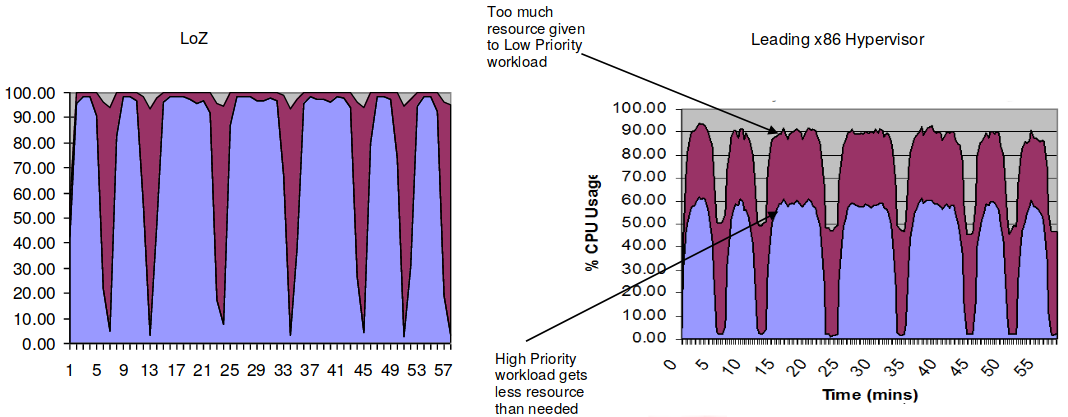
\includegraphics[width=.95\textwidth]{difference-workload-management}
\caption{Workload Management Vergleich mit x86\cite{WorkloadManagement}.}
\label{fig:WorkloadManagement}
\end{figure}

\section{Konsolidierung von Linux Servern}
\label{sec:Konsolidierung}

In Rechenzentren hat man oft das Ziel, die Unterhaltungskosten und Effizienz zu optimieren.
Nicht nur was Platz und Strom angeht sondern auch die Effizienz und Auslastung der Server.
Ein IBM Mainframe mit Linux on z ist prädestiniert dafür komplette Linux Server Farmen auf einer
einzelnen Hardware zu konsolidieren.
Damit es sich überhaupt lohnt eine solche Konsolidierung in Betracht zu ziehen, braucht man eine kritische Masse
an Linux Servern. IBM illustriert diese \textit{kritische Masse} wie folgt:

\begin{figure}[h!]
\centering
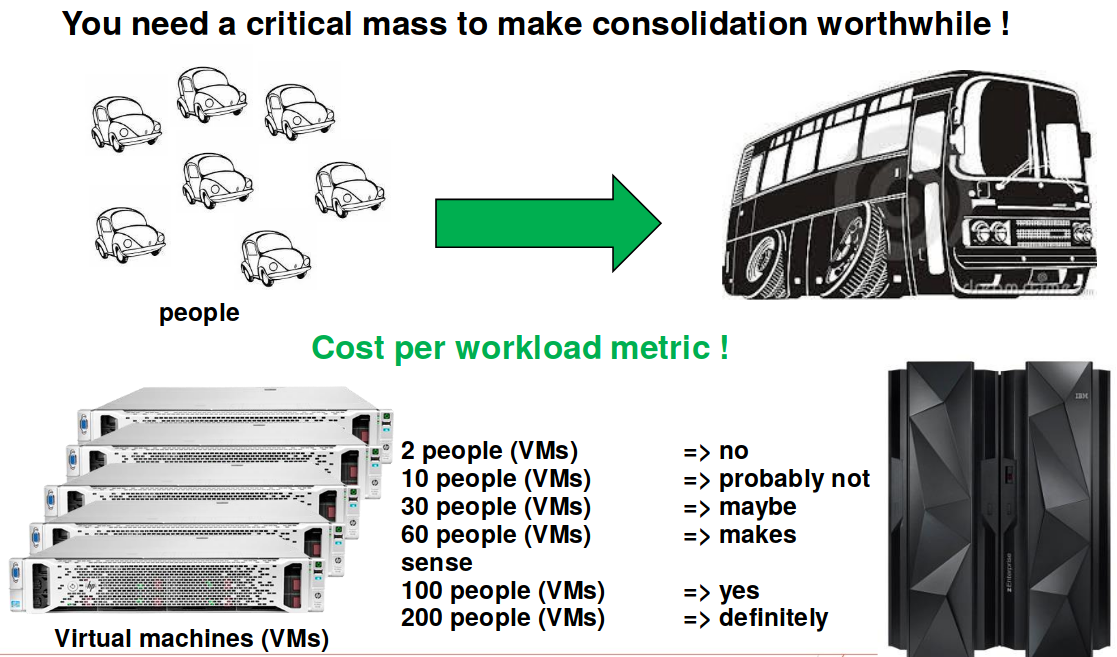
\includegraphics[width=.80\textwidth]{difference-kritische-masse}
\caption{Kritische Masse fuer Konsolidierung\cite{KonsolidierungKritischeMasse}.}
\label{fig:KonsolidierungKritischeMasse}
\end{figure}

IBM hat laut mehreren \textit{Eagle studies} folgende Statistik aufgestellt im Bezug auf x86-Cores zu Linux on z-Cores:

\begin{figure}[h!]
\centering
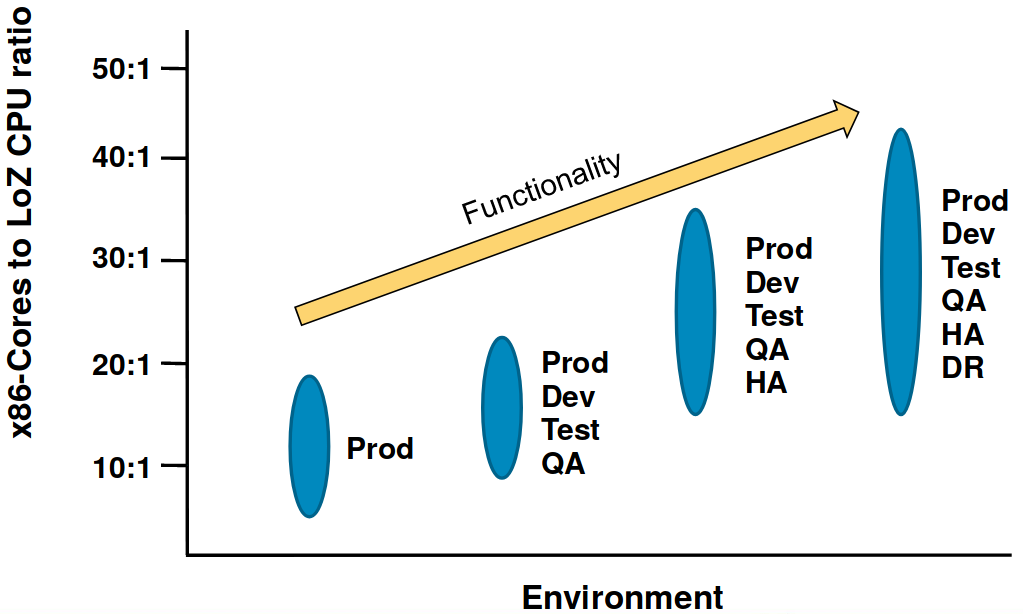
\includegraphics[width=.80\textwidth]{difference-cpu-ratio}
\caption{Rate von x86-Cores zu LoZ-Cores\cite{CPURatio}.}
\label{fig:CPURatio}
\end{figure}

Diese Statistik zeigt, dass umso komplexer ein Environment wird, umso mehr x86-Cores werden im Vergleich zu Linux on z-Cores gebraucht,
damit das Environment die erforderlichen Leistungen erbringen kann.

Dies ist vor allem auf die gute Leistung des Workload Managements zurückzuführen.\footnote{Siehe Abschnitt \ref{sec:WorkloadManagement}}

\section{Kommunikation ueber HiperSockets}
\label{sec:HiperSockets}

Wenn man Applikationssysteme mit mehreren verschiedenen physikalisch getrennten x86 Servern hat, so wird die Kommunikation zwischen diesen meist über Switches mit TCP/IP geroutet. Das Problem dabei ist die Latenzzeit dieser Netzwerkverbindung.
Vor allem bei Systemen bestehend aus Microservices\footnote{man hat also viele kleinere Systeme welche kleine Teilaufgaben einer grösseren Aufgabe übernehmen} kann die Latenzzeit zwischen den Services einen beachtlichen Anteil der gesamt Rechenzeit ausmachen.

Die IBM Mainframes bieten diesen Latenzzeiten mit sogenannten HiperSockets Abhilfe.\cite{HiperSocketsWiki}
HiperSockets bieten \textit{high-speed} \textit{in-memory} TCP/IP Kommunikationskanäle zwischen verschiedenen LPARs an. IBM unterstützt HiperSockets für z/OS, z/VM und auch für Linux on z.

HiperSockets sind ein starkes Argument für die Konsolidierung von x86 Servern auf ein Mainframe. Nicht nur fallen die Kosten für Switches und Kabel nicht sondern es kommt auch noch ein riesen Performance-Vorteil hinzu.

\subsection{HiperSockets als Address-Family}

Der Linux Kernel unterstützt mit der \textit{AF\_IUCV} Address Family eine direkte Kommunikation über HiperSockets zwischen Applikationen laufend auf verschiedenen Linux on z Instanzen.
Für Linux on z in LPARs werden folgende Funktionalitäten unterstützt:
\begin{itemize}
    \item{Mehrere eingehenden \textit{echte} HiperSocket Verbindungen}
    \item{Mehrere ausgehende \textit{echte} HiperSocket Verbindungen}
\end{itemize}
Wird Linux on z unter z/VM betrieben kommen IUCV-Verbinunden\footnote{IUCV steht für Inter-User Communication Vehicle und wird gebraucht, damit mehrere z/VM und Applikationen unter z/VM miteinander kommunizieren können} und keine \textit{echte} HiperSockets zum Einsatz.

Der \textit{AF\_IUCV} Support kann im Linux Kernel über die \textit{CONFIG\_IUCV} und \textit{CONFIG\_AFIUCV} Optionen aktiviert werden.

\begin{figure}[h!]
\centering
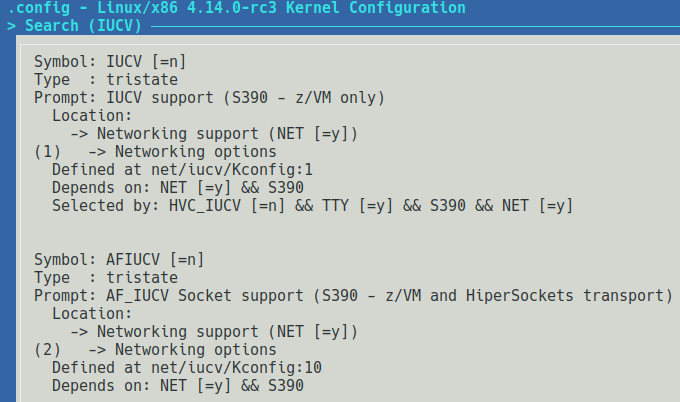
\includegraphics[width=.80\textwidth]{afiucv_menuconfig}
\caption{Linux Kernel \textit{menuconfig} AF\textunderscore IUCV Optionen}
\label{fig:AFIUCVMENUCONFIG}
\end{figure}

Wie bei fast allen Modulen kann der \textit{AF\_IUCV} entweder direkt in den Kernel einkompiliert oder als dynamisches Modul nachgeladen werden.
Das nachladbare Modul heisst \textit{af\_iucv}:\cite{IBMAFIUCV}

\begin{lstlisting}
# modprobe af_iucv
\end{lstlisting}

\section{Call Home - Problem Reporting}

IBM bietet ein Linux Kernel Modul an um, im Falle einer Kernel Panic\footnote{Ein Crash im Kernelspace}, direkt Problem Reports an RETAIN -- ein Datenbank System um die IBM Fieldagents und Kunden zu unterstützen -- zu senden.

Um diese automatischen Problem Reports zu nutzen, müssen folgende Anforderungen erfüllt sein:\cite{IBMCallHome}
\begin{itemize}
    \item{Linux on z muss direkt in einer LPAR installiert sein}
    \item{Der Linux Kernel muss das \textit{SCLP\_ASYNC} device unterstützen}
    \item{Der Kunde braucht ein \textit{Hardware support agreement} mit IBM um die Reports an RETAIN schicken zu dürfen}
\end{itemize}

\subsection{Kernel Konfiguration}

Damit die \textit{Call Home} Funktionalitaet auf Linux Kernel Ebene funktioniert muss die \textit{CONFIG\_SCLP\_ASYNC} Option im Kernel aktiviert sein.

\begin{figure}[h!]
\centering
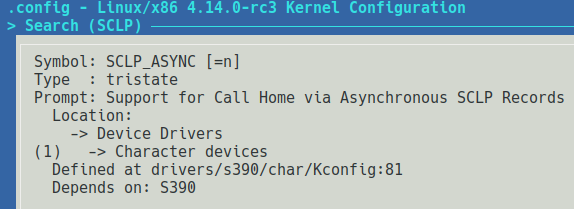
\includegraphics[width=.80\textwidth]{sclp_async_menuconfig}
\caption{Linux Kernel \textit{menuconfig} SCLP\textunderscore ASYNC Optionen}
\label{fig:SCLPASYNC}
\end{figure}

\textit{SCLP\_ASYNC} funktioniert sowohl direkt im Kernel als auch als nachladbares Kernel Module \textit{sclp\_async}:

\begin{lstlisting}
# modprobe sclp_async
\end{lstlisting}

Sobald das Kernel Modul aktiv ist, kann die \textit{Call Home} Funktion übers \textit{procfs} eingeschalten oder wieder ausgeschalten werden:\cite{IBMCallHome}

\begin{lstlisting}
# # Enable call home support
# echo 1 > /proc/sys/kernel/callhome
# # Disable call home support
# echo 0 > /rpco/sys/kernel/callhome
\end{lstlisting}
